%!TEX program = lualatex

\documentclass{VUMIFPSkursinis}
\usepackage{float}
\usepackage{hyperref}
\usepackage{algorithmicx}
\usepackage{algorithm}
\usepackage{algpseudocode}
\usepackage{amsfonts}
\usepackage{amsmath}
\usepackage{bm}
\usepackage{caption}
\usepackage{color}
\usepackage{graphicx}
\usepackage{listings}
\usepackage{subcaption}
\usepackage{wrapfig}
\usepackage{biblatex}
\usepackage{multirow}
\usepackage{microtype}
\usepackage{float}

\usepackage{listings}
\usepackage{xcolor}

\definecolor{codegreen}{rgb}{0,0.6,0}
\definecolor{codegray}{rgb}{0.5,0.5,0.5}
\definecolor{codepurple}{rgb}{0.58,0,0.82}
\definecolor{backcolour}{rgb}{0.95,0.95,0.92}

\lstdefinestyle{mystyle}{
    backgroundcolor=\color{backcolour},
    commentstyle=\color{codegreen},
    keywordstyle=\color{magenta},
    numberstyle=\tiny\color{codegray},
    stringstyle=\color{codepurple},
    basicstyle=\ttfamily\footnotesize,
    breakatwhitespace=false,
    breaklines=true,
    captionpos=b,
    keepspaces=true,
    numbers=left,
    numbersep=5pt,
    showspaces=false,
    showstringspaces=false,
    showtabs=false,
    tabsize=2
}

\lstset{style=mystyle}

% Titulinio aprašas
\university{Vilniaus universitetas}
\faculty{Matematikos ir informatikos fakultetas}
\department{Informatika}
\title{Optimizavimas be apribojimų}
\titleineng{}
\status{3 kurso 1 grupės studentas}
\author{Tomas Kozakas}
% \secondauthor{Vardonis Pavardonis}   % Pridėti antrą autorių
\supervisor{doc. dr. Arvydas Kregždė}
% \addsignatureplaces{} % prideda parašų vietas tituliniame puslapyje
\date{Vilnius - \the\year}

\bibliography{bibliografija}

\begin{document}
\maketitle

\tableofcontents

\section{Įvadas}

Laboratorinio darbo tikslas suprogramuoti gradientinio nusileidimo,
greičiausiojo nusileidimo ir deformuojamo simplekso algoritmus.
Minimizuoti uždavinį, naudojant suprogramuotus algoritmus
pradedant taškuose $X_0 = (0,0)$, $X_1 = (1, 1)$, $X_m = (\frac{a}{10}, \frac{b}{10})$, kur $a = 0$ ir $b = 6$ bei surasti kokie turėtų būti stačiakampio gretasienio formos dėžės matmenys, kad vienetiniam
paviršiaus plotui jos tūris būtų maksimalus.

\section{Užduotys}
\subsection{Užduoties formulavimas}

\begin{enumerate}
  \item Vienetinio dėžės paviršiaus ploto reikalavimas ir vieno kintamojo išraiška per kitus:
        $$x_1 + x_2 + x_3 = 1$$
        $$x_3 = 1 - x_1 - x_2$$
        $x_1, x_2, x_3$ - priekinės ir galinės sienų plotų suma, šoninių sienų plotų suma, viršutinės ir apatinės sienų plotų suma.
  \item Dėžės tūrio pakelto kvadratu (tikslo) funkcija:
        $$V^2 = \left(abc\right)^2$$
        $$V^2 = ab * bc * ac$$
        $$ab = \frac{x_1}{2}, bc = \frac{x_2}{2}, ac = \frac{x_3}{2}$$
        $$V^2 = \frac{x_1x_2x_3}{8}$$
        $$f(x) = V^2 = \frac{x_1x_2(1 - x_1 - x_2)}{8}$$
        $x_1, x_2, x_3$ - priekinės ir galinės sienų plotų suma, šoninių sienų plotų suma, viršutinės ir apatinės sienų plotų suma
        ir $a, b, c$ - dėžes kraštinių ilgiai.
  \item Kad galėtume skaičiuoti tikslo funkcijos minimumą ją reikia padauginti iš $-1$. Taigi:
        $$f(x) = -\frac{x_1x_2(1 - x_1 - x_2)}{8}$$
  \item Funkcijos gradientas:
        $$\frac{\partial }{\partial \:x_1}\left(-\frac{x_1x_2\left(1\:-\:x_1\:-\:x_2\right)}{8}\right) = -\frac{x_2\left(-2x_1-x_2+1\right)}{8}$$
        $$\frac{\partial }{\partial \:x_2}\left(-\frac{x_1x_2\left(1\:-\:x_1\:-\:x_2\right)}{8}\right) = -\frac{x_1\left(1-x_1-2x_2\right)}{8}$$
        $$\nabla f(X) = \left(-\frac{x_2\left(-2x_1-x_2+1\right)}{8},-\frac{x_1\left(1-x_1-2x_2\right)}{8}\right)$$
  \item Tikslo ir gradiento funkcijų reikšmės pradiniuose taškuose:
        \begin{table}[H]
          \centering
          \caption{$f(X)$ ir $\nabla f(X)$ reikšmės pradiniuose taškuose.}
          \begin{tabular}{l c c}
            \hline\hline
            Taškas                         & $f(X)$  & $\nabla f(X)$    \\ [0.5ex]
            \hline
            $(0, 0)$                       & 0       & (0, 0)       \\
            $(1, 1)$                       & 0.125   & (0.25, 0.25)     \\
            $({0}, \frac{6}{10})$ & 0 & (-0.03, 0) \\ [1ex]
            \hline
          \end{tabular}
          \label{table:stpoints}
        \end{table}
\end{enumerate}

\begin{figure}[H]
  \centering
  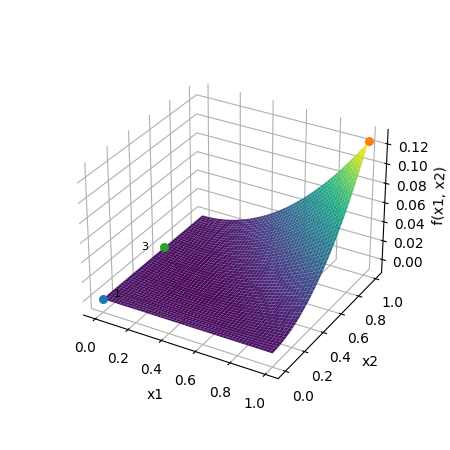
\includegraphics[width=10cm]{img/starting_points.png}
  \caption{Tikslo funkcijos vizualizavimas bei pradiniai taškai.}
  \label{img:start-plot}
\end{figure}

\subsection{Gradientinio nusileidimo algoritmas}

Gradientinio nusileidimo algoritmas (\ref{code:grad-des} pr.).
Algoritmas buvo paleistas iš 3 taškų: $(1, 1)$, $(0, 0)$, $(0, 0.6)$.
Pagal algoritmo veikimo rezultatus buvo sudaryti grafikai
(\ref{img:grad-des-3d-11} - \ref{img:grad-des-3d-00} pav.).
Algoritmo veikimo rezultatai buvo surašyti į lentelę (\ref{table:grad-des} lent.).
Kai pradinis taškas yra $(0, 0)$ algoritmas negali susirasti minimumo,
nes tame taške funkcijos gradientas yra lygus nuliui.
Kai pradinis taškas yra $(1, 1)$ algoritmas padaro 28 iteracijas ir artėja tiesiai prie minimumo.
Kai pradinis taškas yra $(0, 0.6)$ algoritmui jau reikia padaryti daugiau žingsnių.

\begin{table}[H]
  \centering
  \caption{Gradientinio nusileidimo algoritmo veikimo rezultatai.}
  \begin{tabular}{l c c}
    \hline\hline
    Taškas                         & $f(X)$ išk. sk. & Iteracijų sk. \\ [0.5ex]
    \hline
    $(0, 0)$                        & 2               & 1             \\
    $(1, 1)$                        & 56              & 28            \\
    $({0}, \frac{6}{10})$           & 148             & 74            \\ [1ex]
    \hline
  \end{tabular}
  \label{table:grad-des}
\end{table}

% 1 1
\begin{figure}[H]
  \centering
  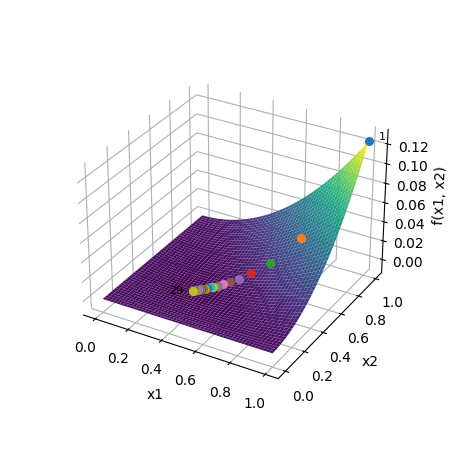
\includegraphics[width=10cm]{img/gradient_descent_3d_[1.0,1.0].png}
  \caption{Gradientinio nusileidimo algoritmo 3d vizualizacija. Pradinis taškas $[1, 1]$}
  \label{img:grad-des-3d-11}
\end{figure}

\begin{figure}[H]
  \centering
  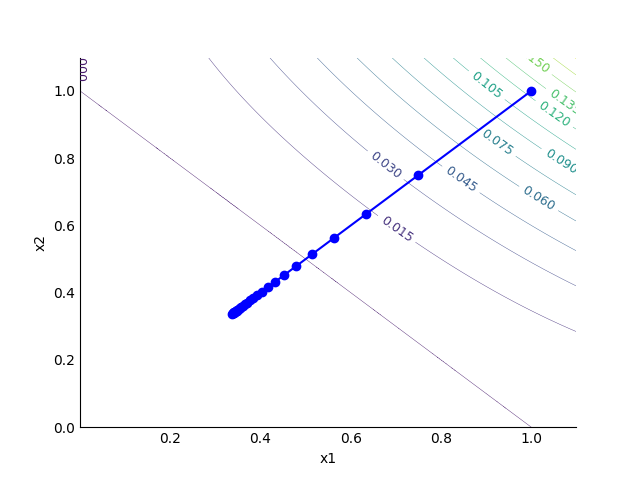
\includegraphics[width=10cm]{img/gradient_descent_contour_[1.0,1.0].png}
  \caption{Gradientinio nusileidimo algoritmo kontūrinė vizualizacija. Pradinis taškas $[1, 1]$}
  \label{img:grad-des-co-11}
\end{figure}

% 0 0.6
\begin{figure}[H]
  \centering
  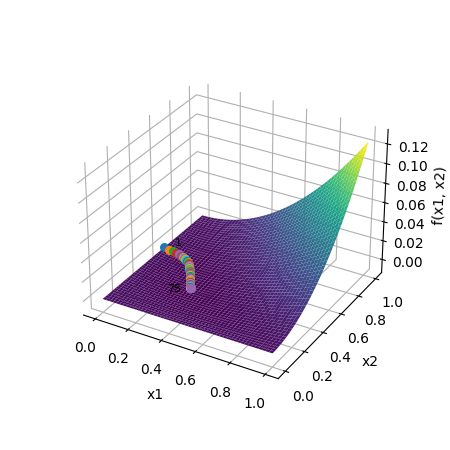
\includegraphics[width=10cm]{img/gradient_descent_3d_[0.0,0.6].png}
  \caption{Gradientinio nusileidimo algoritmo 3d vizualizacija. Pradinis taškas $[0, 0.6]$}
  \label{img:grad-des-3d-69}
\end{figure}

\begin{figure}[H]
  \centering
  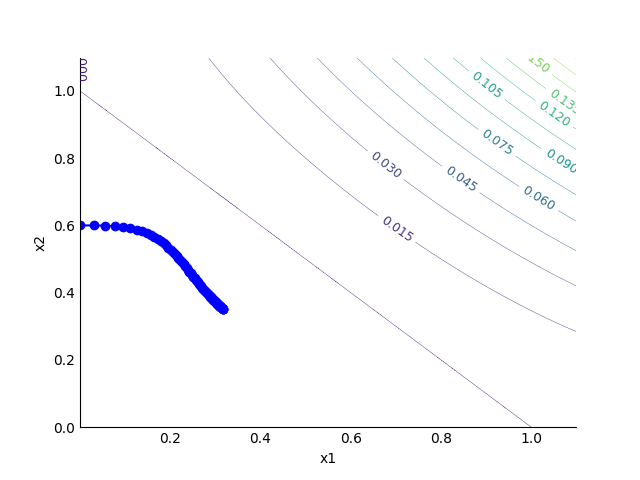
\includegraphics[width=10cm]{img/gradient_descent_contour_[0.0,0.6].png}
  \caption{Gradientinio nusileidimo algoritmo kontūrinė vizualizacija. Pradinis taškas $[0, 0.6]$}
  \label{img:grad-des-co-69}
\end{figure}

% 0 0
\begin{figure}[H]
  \centering
  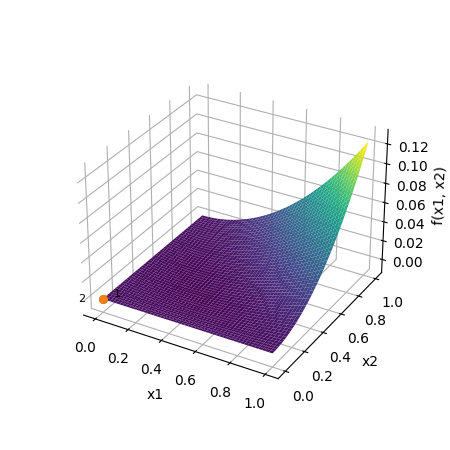
\includegraphics[width=10cm]{img/gradient_descent_3d_[0.0,0.0].png}
  \caption{Gradientinio nusileidimo algoritmo 3d vizualizacija. Pradinis taškas $[0, 0]$}
  \label{img:grad-des-3d-00}
\end{figure}

\pagebreak
\subsection{Greičiausiojo nusileidimo algoritmas}

Greičiausiojo nusileidimo algoritmas, skirtingai nei gradientinio, sprendžia papildomą optimizavimo uždavinį, naudodamas Auksinio pjūvio algoritmą, kad nustatyti žingsnį. Nors jis negali rasti minimumo iš taško $(0, 0)$ dėl nulinio gradiento (\ref{img:steep-des-3d-00} pav.), jis greitai suranda minimumą iš taško $(1, 1)$ (\ref{img:steep-des-3d-11}  pav.). Tačiau, pradedant $(0, 0.6)$, reikia daugiau iteracijų ir funkcijos iškvietimų (\ref{img:steep-des-3d-69} pav.).

\begin{table}[H]
  \centering
  \caption{Greičiausiojo nusileidimo algoritmo veikimo rezultatai.}
  \begin{tabular}{l c c}
    \hline\hline
    Taškas                         & $f(X)$ išk. sk. & Iteracijų sk. \\ [0.5ex]
    \hline
    $(0, 0)$                       & 2               & 1             \\
    $(1, 1)$                       & 4               & 2             \\
    $({0}, \frac{6}{10})$ & 44              & 22            \\ [1ex]
    \hline
  \end{tabular}
  \label{table:steep-des}
\end{table}

\begin{table}[H]
  \centering
  \caption{Greičiausiojo nusileidimo papildomų uždavinių sprendimo statistika.}
  \begin{tabular}{l c c}
    \hline\hline
    Taškas                         & $f(X)$ išk. sk. & Iteracijų sk. \\ [0.5ex]
    \hline
    $(0, 0)$                       & 18              & 20            \\
    $(1, 1)$                       & 36              & 40            \\
    $({0}, \frac{0}{6})$ & 440             & 396           \\ [1ex]
    \hline
  \end{tabular}
  \label{table:steep-des-add}
\end{table}

% 1 1
\begin{figure}[H]
  \centering
  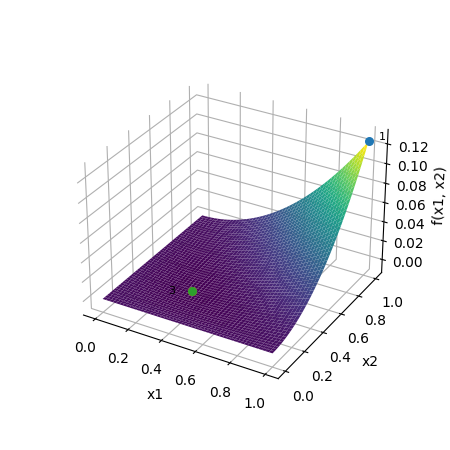
\includegraphics[width=10cm]{img/steepest_descent_3d_[1.0,1.0].png}
  \caption{Greičiausiojo nusileidimo algoritmo 3d vizualizacija,Pradinis taškas $[1, 1]$}
  \label{img:steep-des-3d-11}
\end{figure}

\begin{figure}[H]
  \centering
  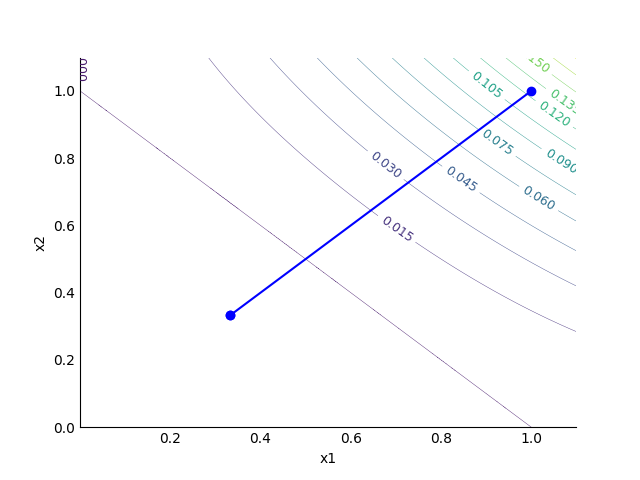
\includegraphics[width=10cm]{img/steepest_descent_contour_[1.0,1.0].png}
  \caption{Greičiausiojo nusileidimo algoritmo kontūrinė vizualizacija. Pradinis taškas $[1, 1]$}
  \label{img:steep-des-co-11}
\end{figure}

% 0 0.6
\begin{figure}[H]
  \centering
  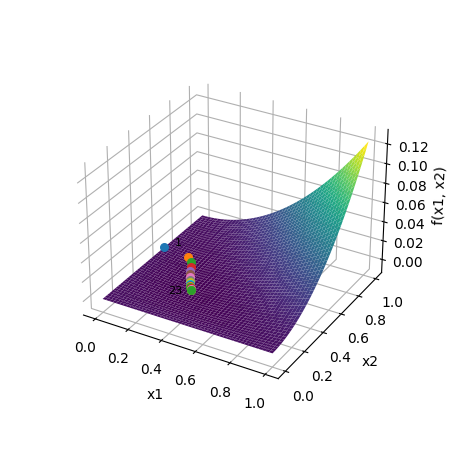
\includegraphics[width=10cm]{img/steepest_descent_3d_[0.0,0.6].png}
  \caption{Greičiausiojo nusileidimo algoritmo 3d vizualizacija. Pradinis taškas $[0, 0.6]$}
  \label{img:steep-des-3d-69}
\end{figure}

\begin{figure}[H]
  \centering
  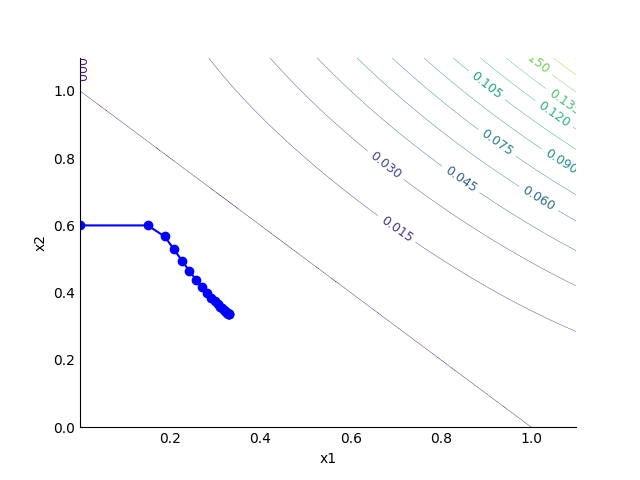
\includegraphics[width=10cm]{img/steepest_descent_contour_[0.0,0.6].png}
  \caption{Greičiausiojo nusileidimo algoritmo kontūrinė vizualizacija. Pradinis taškas $[0, 0.6]$}
  \label{img:steep-des-co-69}
\end{figure}

% 0 0
\begin{figure}[H]
  \centering
  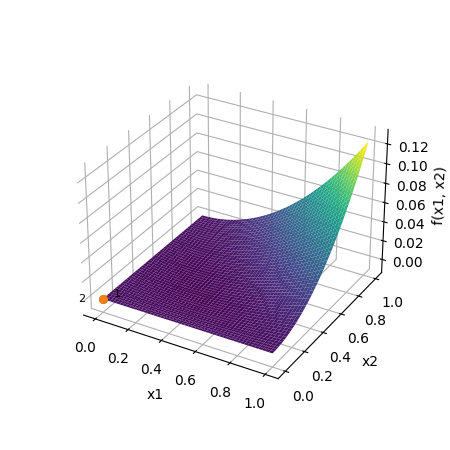
\includegraphics[width=10cm]{img/steepest_descent_3d_[0.0,0.0].png}
  \caption{Greičiausiojo nusileidimo algoritmo 3d vizualizacija. Pradinis taškas $[0, 0]$}
  \label{img:steep-des-3d-00}
\end{figure}

\subsection{Deformuojamo simplekso algoritmas}

Deformuojamo simplekso algoritmas nenaudoja funkcijos gradiento skaičiavimams ir dėl to jis
gali surasti funkcijos minimumą net ir iš taško, kur funkcijos
gradientas yra lygus nuliui (\ref{img:nel-mead-00} pav.).
Algoritmo veikimo rezultatai yra atvaizduoti \ref{table:nel-mead} lentelėje.
Grafikai atvaizduoja visas algoritmo iteracijas nuo pirmos iki paskutinės.
Kiekvienos iteracijos taškai sudaro tam tikros spalvos trikampį ant grafiko
(\ref{img:nel-mead-11} pav., \ref{img:nel-mead-69} pav., \ref{img:nel-mead-00} pav.).
Deformuojamo simplekso algoritmo realizacija galima peržiūrėti \ref{code:nm} priede.

\begin{table}[H]
  \centering
  \caption{Deformuojamo simplekso algoritmo veikimo rezultatai.}
  \begin{tabular}{l c c}
    \hline\hline
    Taškas                         & $f(X)$ išk. sk. & Iteracijų sk. \\ [0.5ex]
    \hline
    $(0, 0)$                       & 71              & 25            \\
    $(1, 1)$                       & 101             & 35            \\
    $({0}, \frac{6}{10})$ & 76             & 26            \\ [1ex]
    \hline
  \end{tabular}
  \label{table:nel-mead}
\end{table}

% 1 1
\begin{figure}[H]
  \centering
  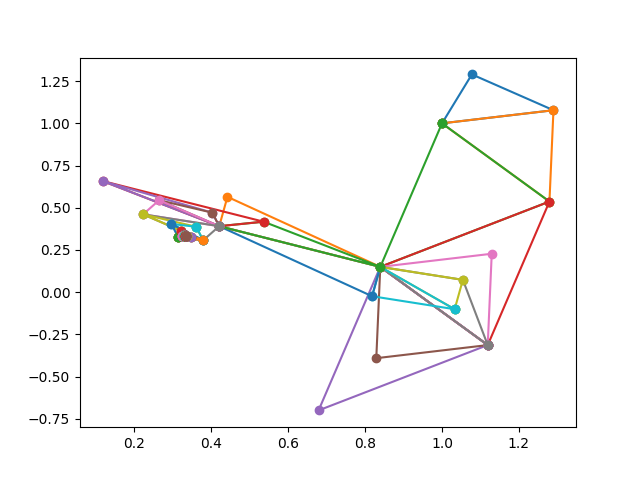
\includegraphics[width=10cm]{img/nelder_mead_better_triangles_[1.0,1.0].png}
  \caption{Deformuojamo simplekso algoritmo vizualizacija pradiniame taške $[1, 1]$}
  \label{img:nel-mead-11}
\end{figure}

% 0 0.6
\begin{figure}[H]
  \centering
  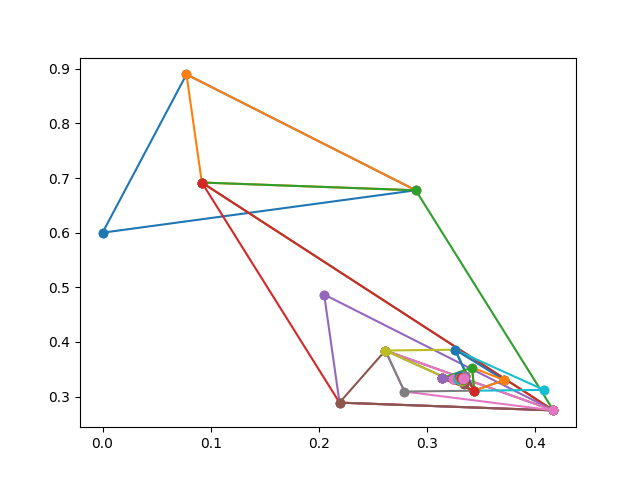
\includegraphics[width=10cm]{img/nelder_mead_better_triangles_[0.0,0.6].png}
  \caption{Deformuojamo simplekso algoritmo vizualizacija pradiniame taške $[0, 0.6]$}
  \label{img:nel-mead-69}
\end{figure}

% 0 0
\begin{figure}[H]
  \centering
  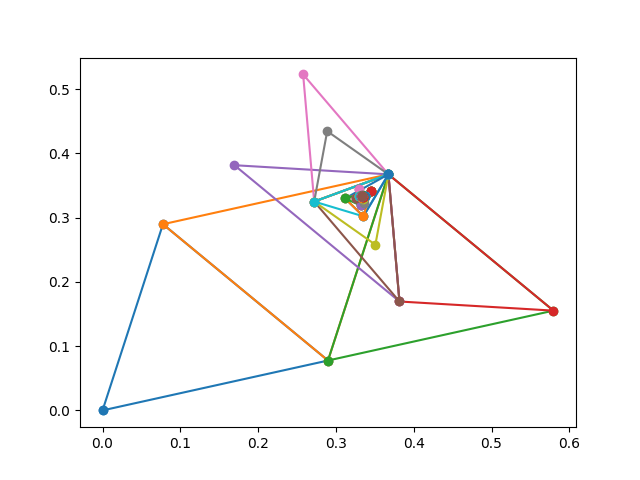
\includegraphics[width=10cm]{img/nelder_mead_better_triangles_[0.0,0.0].png}
  \caption{Deformuojamo simplekso algoritmo vizualizacija pradiniame taške $[0, 0]$}
  \label{img:nel-mead-00}
\end{figure}

\section{Rezultatai, palyginimas ir išvados}

Lyginant rezultatus, gradientinio ir greičiausiojo nusileidimo metodai nepasisekė rasti minimumo su nuliniu gradientu. Greičiausiojo nusileidimo metodo efektyvumas greitai mažėja, nes jis reikalauja,
kad būtų sprendžiamas papildomas optimizavimo uždavinys, bet yra atvejų, kai
jis gali surasti minimumą vos per 2 iteracijas (\ref{table:compar-11} lent.). Deformuojamo simplekso metodas visada suranda minimumą. Taipat po minimizavimo užduoties atlikimo, išsiaiškinau, kad galutinė optimali dėžės forma siekiant maks. tūrio: \textit{kubas}.

\begin{table}[H]
  \centering
  \caption{Rezultatų palyginimas taške $(0, 0)$.}
  \resizebox{\textwidth}{!}{\begin{tabular}{l c c c c}
      \hline\hline
      Pavadinimas             & $f(X)$ išk. sk. & It. sk. & Atrastas taškas            & Funk. min. įvertis \\ [0.5ex]
      \hline
      Gradientinio nus. alg.  & 2               & 1       & $(0, 0)$                   & 0                  \\
      Greičiausiojo nus.      & 2 + 20          & 1 + 18  & $(0, 0)$                   & 0                  \\
      Deformuojamo simp. alg. & 71              & 25      & $(0.33365361, 0.33386664)$ & -0.00462960636    \\ [1ex]
      \hline
    \end{tabular}}
  \label{table:compar-00}
\end{table}

\begin{table}[H]
  \centering
  \caption{Rezultatų palyginimas taške $(1, 1)$.}
  \resizebox{\textwidth}{!}{\begin{tabular}{l c c c c}
      \hline\hline
      Pavadinimas            & $f(X)$ išk. sk. & It. sk. & Atrastas taškas            & Funk. min. įvertis \\ [0.5ex]
      \hline
      Gradientinio nus. alg. & 56              & 28      & $(0.33785945, 0.33785945)$ & -0.0046270457
      \\
      Greičiausiojo nus.     & 4 + 40          & 2 + 36  & $(0.33331962, 0.33331962)$ & -0.00462962
      \\
      Deformuojamo sim. alg. & 101             & 35      & $(0.333646, 0.33316277)$ & -0.004629626      
      \\ [1ex]
      \hline
    \end{tabular}}
  \label{table:compar-11}
\end{table}

\begin{table}[H]
  \centering
  \caption{Rezultatų palyginimas taške $(0, 0.6)$.}
  \resizebox{\textwidth}{!}{\begin{tabular}{l c c c c}
      \hline\hline
      Pavadinimas            & $f(X)$ išk. sk. & It. sk.  & Atrastas taškas            & Funk. min. įvertis \\ [0.5ex]
      \hline
      Gradientinio nus. alg. & 148             & 74       & $(0.31792924, 0.35009072)$ & -0.00461884
      \\
      Greičiausiojo nus.     & 40 + 440        & 22 + 396 & $(0.33103112, 0.33566213)$ & -0.0046294
      \\
      Deformuojamo s. alg.   & 76             & 26       & $(0.33335288, 0.33365688)$ & -0.00462962
      \\ [1ex]
      \hline
    \end{tabular}}
  \label{table:compar-69}
\end{table}

\section{Priedai}

\begin{lstlisting}[language=Python,caption={Gradientinio nusileidimo algoritmo realizacija su Python},label={code:grad-des}]
  def gradient_descent(gradf, start, learning_rate=1, tolerance=0.001):
  steps = [start]  # stat tracing
  function_uses = 0
  xi = start

  while True:
      gradxi = gradf(xi)  # Find gradient at point X_i
      function_uses += 2

      xi = xi - learning_rate * gradxi  # Find X_i+1 = X_i - gamma * gradf(X_i)
      steps.append(xi)  # stat tracing

      if np.linalg.norm(learning_rate * gradxi) < tolerance:
          break
  return steps, xi, function_uses
\end{lstlisting}

\begin{lstlisting}[language=Python,caption={Greičiausiojo nusileidimo algoritmo realizacija su Python},label={code:steep-des}]
  def golden_section(xi, gradxi, func, l=0, r=5, deltax=0.001):
  tau = (-1 + math.sqrt(5)) / 2
  stats = {"function_uses": 0, "iterations": 0}

  # Step 1
  L = r - l
  point1 = r - tau * L
  value_of_function_at_point1 = func(xi + point1 * (-gradxi))
  stats["function_uses"] += 1
  point2 = l + tau * L
  value_of_function_at_point2 = func(xi + point2 * (-gradxi))
  stats["function_uses"] += 1

  while True:
      stats["iterations"] += 1
      # Step 2
      if value_of_function_at_point2 < value_of_function_at_point1:
          l = point1
          L = r - l
          point1 = point2
          value_of_function_at_point1 = value_of_function_at_point2

          point2 = l + tau * L
          value_of_function_at_point2 = func(xi + point2 * (-gradxi))
          stats["function_uses"] += 1
      # Step 3
      else:
          r = point2
          L = r - l
          point2 = point1
          value_of_function_at_point2 = value_of_function_at_point1

          point1 = r - tau * L
          value_of_function_at_point1 = func(xi + point1 * (-gradxi))
          stats["function_uses"] += 1
      # Step 4
      if L < deltax:
          return (point1 + point2) / 2, stats


def steepest_descent(f, gradf, start, tolerance=0.001):
  steps = [start]  # stat tracing
  stats_additional = {"function_uses": 0, "iterations": 0, "count": 0}
  function_uses = 0
  xi = start

  while True:
      gradxi = gradf(xi)  # Find gradient at point X_i
      function_uses += 2

      learning_rate, stats = golden_section(
          xi, gradxi, f
      )  # Find gamma such: arg min_gamma >= 0 f(X_i - gamma * gradf(X_i))

      stats_additional["function_uses"] += stats["function_uses"]
      stats_additional["iterations"] += stats["iterations"]
      stats_additional["count"] += 1

      xi = xi - learning_rate * gradxi  # Find X_i+1 = X_i - gamma * gradf(X_i)
      steps.append(xi)  # stat tracing

      if np.linalg.norm(learning_rate * gradxi) < tolerance:
          break
  return steps, xi, function_uses, stats_additional
\end{lstlisting}

\begin{lstlisting}[language=Python,caption={Deformuojamo simplekso algoritmo realizacija su Python},label={code:nm}]
  def generate_points(
    f,
    starting_point,
    alpha=0.3
):  # Alpha is basically the length of the side of the initial simplex
    x0 = np.array(starting_point)
    n = len(x0)
    X = [x0]
    sqrt2 = math.sqrt(2)

    for i in range(n):
        si = []
        for j in range(n):
            if i == j:
                si.append((math.sqrt(n + 1) - 1) / (n * sqrt2) * alpha)
            else:
                si.append((math.sqrt(n + 1) + n - 1) / (n * sqrt2) * alpha)
        X.append(x0 + si)

    # Form a list of dictionaries with point coordinates and the value of a function
    return [{
        "coords": np.array(x[0]),
        "value": x[1]
    } for x in zip(X, [f(x) for x in X])]


def find_centroid(f, points, n, worst_points_index):
    centroid_coords = 1 / n * sum(
        [v['coords'] for i, v in enumerate(points) if i != worst_points_index])
    return {"coords": centroid_coords, "value": f(centroid_coords)}


def step(f, points, centroid, worst_points_index, alpha):
    new_point_coords = centroid['coords'] + alpha * (
        centroid['coords'] - points[worst_points_index]['coords'])
    return {"coords": new_point_coords, "value": f(new_point_coords)}


def find_worst_points_index(points):
    return np.array([point['value'] for point in points]).argmax()


def find_second_worst_points_index(points):
    worst_points_index = find_worst_points_index
    return np.array([
        v['value'] for i, v in enumerate(points) if i != worst_points_index
    ]).argmax()


def find_best_points_index(points):
    return np.array([point['value'] for point in points]).argmin()


def shrink(f, points, gamma=0.5):
    X = []

    for i, x in enumerate(points):
        if i == find_best_points_index(points):
            X.append(x)
            continue

        best_point = points[find_best_points_index(points)]
        x_coords = best_point['coords'] + gamma * (x['coords'] -
                                                   best_point['coords'])
        X.append({"coords": x_coords, "value": f(x_coords)})

    return X


def nelder_mead(f, starting_point, tolerance=0.001):
    # Stat tracing
    triangles = []
    function_calls = 0

    # Generate Simplex Points
    simplex = generate_points(f, starting_point)
    function_calls += len(simplex)

    n = len(simplex) - 1  # Number of variables

    while True:
        # Select Worst Point
        worst_points_index = find_worst_points_index(simplex)

        # Find Centroid
        centroid = find_centroid(f, simplex, n, worst_points_index)
        function_calls += 1

        # Reflection
        xr = step(f, simplex, centroid, worst_points_index, 1)
        function_calls += 1

        triangles.append(copy.deepcopy(simplex))  # Stats

        # Try Expansion
        if xr['value'] <= simplex[find_best_points_index(
                simplex)]['value']:  # F(x_r) <= F(x^(0))
            xe = step(f, simplex, centroid, worst_points_index, 2)
            function_calls += 1

            if xe['value'] <= simplex[find_best_points_index(
                    simplex)]['value']:  # F(x_e) <= F(x^(0))
                simplex[worst_points_index] = xe
            else:
                simplex[worst_points_index] = xr
        # Reflected is fine
        elif xr['value'] <= simplex[find_second_worst_points_index(
                simplex)]['value']:
            simplex[worst_points_index] = xr
        # Inside contraction
        elif xr['value'] >= simplex[worst_points_index]['value']:
            xic = step(f, simplex, centroid, worst_points_index, -0.5)
            function_calls += 1

            if xic['value'] <= simplex[worst_points_index]['value']:
                simplex[worst_points_index] = xic
            # Shrink
            else:
                simplex = shrink(f, simplex)
                function_calls += n
        # Outside contraction
        else:
            xoc = step(f, simplex, centroid, worst_points_index, 0.5)
            function_calls += 1

            if xoc['value'] <= simplex[worst_points_index]['value']:
                simplex[worst_points_index] = xoc
            # Shrink
            else:
                simplex = shrink(f, simplex)
                function_calls += n

        if np.linalg.norm(simplex[find_worst_points_index(simplex)]['coords'] -
                          simplex[find_best_points_index(simplex)]['coords']
                          ) <= tolerance:
            break

    return simplex, triangles, function_calls
\end{lstlisting}

\end{document}
